\documentclass{standalone}

\usepackage{tikz,pgf,pgfplots,circuitikz}
\pgfplotsset{compat=1.15}
\usetikzlibrary{intersections,arrows.meta,angles,calc,3d,decorations.pathmorphing}

\usepackage{amssymb,amsfonts,amsthm,mathtools}
\usepackage{physics,braket,bm}

\begin{document}  
  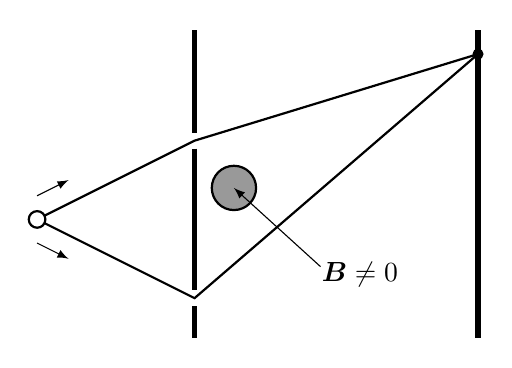
\begin{tikzpicture}
    \draw[thick](-2,0)--(0,1)--(3.6,2.1);
    \draw[thick](-2,0)--(0,-1)--(3.6,2.1);
    \draw[line width=2pt](0,2.4)--(0,1.1);
    \draw[line width=2pt](0,0.9)--(0,-0.9);
    \draw[line width=2pt](0,-1.5)--(0,-1.1);    
    \draw[line width=2pt](3.6,2.4)--(3.6,-1.5);

    \fill[white](-2,0)circle(3pt);
    \draw[thick](-2,0)circle(3pt);

    \fill[black](3.6,2.1)circle(2pt);

    \draw[-latex,thin](-2,0.3)--(-1.6,0.5);
    \draw[-latex,thin](-2,-0.3)--(-1.6,-0.5);

    \fill[black,opacity=0.4](0.5,0.4)circle(8pt);
    \draw[thick](0.5,0.4)circle(8pt);

    \draw[-latex](1.6,-0.6)--(0.5,0.4);
    \draw(2.1,-0.7)node{$\bm{B}\neq0$};
  \end{tikzpicture}
\end{document}
